\documentclass[12pt,a4paper]{article}

\usepackage[utf8]{inputenc}
\usepackage[T1]{fontenc}
\usepackage{amsmath,amssymb,amsfonts}
\usepackage{physics}
\usepackage{booktabs}
\usepackage{array}
\usepackage[margin=1in]{geometry}
\usepackage{hyperref}
\usepackage{graphicx}
\usepackage{float}
\usepackage{enumitem}
\usepackage{authblk}
\usepackage{abstract}
\usepackage{titlesec}

\hypersetup{
  colorlinks=true,
  linkcolor=blue,
  citecolor=blue,
  urlcolor=blue
}

\title{\textbf{The Dirac Equation as a Kuramoto Phase-Synchronization System:}\\[6pt]
\large Mass as Chiral Coupling, Measurement as Re-Synchronization,\\
and a Single-World Account of Decoherence}

\author[1]{Claude Opus 4.6}
\author[2]{J.\ Olddog}
\affil[1]{Anthropic, Large Language Model}
\affil[2]{Independent Research}

\date{Correspondence: \texttt{rayolddog} (GitHub)\\[4pt]
\textit{Preprint --- not yet peer reviewed}}

\begin{document}

\maketitle

\begin{abstract}
We demonstrate that the Dirac equation, written in the chiral (Weyl) basis, has the
mathematical structure of a Kuramoto phase-synchronization system. The left- and
right-handed chiral sectors act as coupled oscillators, with the mass term playing
the role of the Kuramoto coupling constant: $K = m$. For massless particles ($K = 0$)
the chiral clocks are permanently decoupled; for massive particles ($K > 0$) they
synchronize, and the synchronized state is what we identify as a particle with
definite rest mass. The Higgs--Yukawa interaction is the mechanism that sets $K$:
$K = y_f \cdot \langle\phi\rangle = m$.

This identification has three consequences developed in this paper. First, a
non-relativistic phase-clock model using only the temporal (large) Dirac component
yields a Bell correlation $E(a,b) = -\tfrac{1}{2}\cos(a-b)$, below even the classical Bell bound.
When the spatial (small) component is included via the relativistic mixing angle
$\theta_{\mathrm{rel}} = \arcsin(v/c)$, the full quantum result $E(a,b) = -\cos(a-b)$ is recovered
exactly through a three-term decomposition $E = E_{LL} + E_{SS} + E_{LS}$.

Second, quantum measurement is re-interpreted as Kuramoto re-synchronization: a
particle initially synchronized with its entangled partner re-synchronizes to the
macroscopic detector bulk, whose overwhelmingly greater Kuramoto inertia
($M_{\mathrm{detector}} \gg m_{\mathrm{particle}}$) forces conformity. Decoherence is not merely loss of
phase coherence with the partner---it is the positive process of gaining coherence
with the bulk. The Kuramoto framework provides the dynamical mechanism underlying
this process.

Third, we propose a single-world energy accounting: the residual wavefunction
amplitude that does not couple to the detector thermalizes into the electromagnetic
vacuum as low-frequency radiation. No branches are created. The energy is conserved
within a single world.

We present this framework as an interpretive reframing of standard quantum mechanics
---not a modification of its predictions. The Dirac equation is unchanged; Bell's
theorem is not challenged. What is new is the identification of mass as
synchronization coupling, measurement as re-synchronization dynamics, and
decoherence as a Kuramoto process with a specific physical mechanism.
\end{abstract}

\newpage

%% ============================================================
\section{Introduction}

\subsection{The Measurement Problem}

The quantum measurement problem remains the most consequential unsolved problem in
the foundations of physics. The Schr\"odinger equation is linear and deterministic,
yet measurements have definite outcomes. A system in superposition
$\psi = \alpha|0\rangle + \beta|1\rangle$, entangled with a detector, produces
\begin{equation}
|\Psi\rangle = \alpha|0\rangle|D_0\rangle + \beta|1\rangle|D_1\rangle
\end{equation}
The equation has no mechanism to select one outcome. The Born rule---$P(0) = |\alpha|^2$---is postulated, not derived.

The three mainstream responses each carry significant costs. Copenhagen introduces
a mysterious collapse with no physical mechanism. Everett's many-worlds~\cite{everett1957} preserves
unitarity at the cost of infinite unobservable branches. Bohmian mechanics~\cite{bohm1952} accepts
explicit nonlocality through a physically inert pilot wave.

\subsection{What Is Missing: A Dynamical Mechanism for Decoherence}

Environmental decoherence~\cite{zurek2003} has become the standard framework for
understanding how quantum superpositions become effectively classical. It
successfully explains the emergence of preferred ``pointer states'' and the
suppression of off-diagonal density matrix elements through interaction with
environmental degrees of freedom.

Yet decoherence theory describes \emph{what happens} without specifying the dynamical
mechanism by which it happens. The environment is treated as an abstract bath
with many degrees of freedom. This paper proposes that the Kuramoto
phase-synchronization model---specifically, as it appears in the structure of the
Dirac equation itself---provides this missing mechanism.

\subsection{The Proposal in Brief}

We make three claims, in decreasing order of mathematical rigor:

\begin{enumerate}
\item \textbf{The Dirac mass term is a Kuramoto coupling} (Section~2). This is a
  mathematical identification: the chiral Dirac equation has exactly the structure
  of two coupled Kuramoto oscillators with $K = m$. This is the strongest claim and
  is verifiable by inspection.

\item \textbf{Measurement is re-synchronization} (Section~4). When a particle interacts
  with a macroscopic detector, the Kuramoto dynamics drive the particle's phase
  from coherence with its entangled partner to coherence with the detector bulk.
  This provides a physical picture of decoherence. This is an interpretive claim.

\item \textbf{Residual energy thermalizes in a single world} (Section~5). The
  wavefunction amplitude not absorbed by the detector dissipates as thermal
  radiation into the vacuum. No branches are created. This is a speculative but
  physically motivated proposal.
\end{enumerate}

\subsection{What This Paper Does Not Claim}

We state clearly at the outset:

\begin{itemize}
\item We do not challenge Bell's theorem~\cite{bell1964}. The quantum correlations $E(a,b) = -\cos(a-b)$
  arise from the entangled singlet state and the full Dirac spinor structure---standard quantum mechanics.
\item We do not modify the Dirac equation or any of its predictions.
\item We do not propose new physics. We propose a new \emph{mechanism} for known physics.
\item The framework is an interpretation---it may or may not generate distinguishable
  predictions from standard decoherence theory. We are honest about this throughout.
\end{itemize}

%% ============================================================
\section{The Dirac Equation as a Kuramoto System}

\subsection{Chiral Decomposition}

In the Weyl (chiral) basis, the Dirac spinor decomposes into two two-component
Weyl spinors:
\begin{equation}
\psi = \begin{pmatrix} \psi_L \\ \psi_R \end{pmatrix}
\end{equation}
The Dirac equation separates into two coupled equations:
\begin{align}
i\bar{\sigma}^\mu \partial_\mu \psi_L &= m\,\psi_R \tag{1a}\\
i\sigma^\mu \partial_\mu \psi_R &= m\,\psi_L \tag{1b}
\end{align}
where $\sigma^\mu = (I, \boldsymbol{\sigma})$ and $\bar{\sigma}^\mu = (I, -\boldsymbol{\sigma})$ are the Weyl matrices.

\textbf{For $m = 0$ (massless):} Equations (1a) and (1b) decouple entirely. $\psi_L$ and $\psi_R$
satisfy independent equations. The particle has definite chirality and no rest
frame. Photons and massless-limit neutrinos are in this category.

\textbf{For $m \neq 0$ (massive):} The equations couple $\psi_L$ to $\psi_R$ and vice versa. Neither
chirality state is stable alone; the physical particle is a superposition of both.
The coupling strength is exactly $m$.

\subsection{The Kuramoto Identification}

The standard Kuramoto model~\cite{kuramoto1975} describes the phase dynamics of $N$
coupled oscillators:
\begin{equation}
\frac{d\phi_i}{dt} = \omega_i + \frac{K}{N}\sum_j \sin(\phi_j - \phi_i)
\end{equation}
Writing $\psi_L = \rho_L^{1/2}\,e^{i\phi_L}\,\chi_L$ and $\psi_R = \rho_R^{1/2}\,e^{i\phi_R}\,\chi_R$, the
phase dynamics extracted from Equations~(1) yield:
\begin{align}
\frac{d\phi_L}{dt} &= \omega_L + K\sin(\phi_R - \phi_L + \delta_{CP}) \tag{2a}\\
\frac{d\phi_R}{dt} &= \omega_R + K\sin(\phi_L - \phi_R - \delta_{CP}) \tag{2b}
\end{align}
where the coupling constant is:
\begin{equation}
\boxed{K = y_f \cdot |\langle\phi\rangle| = y_f \cdot \frac{v}{\sqrt{2}} = m} \tag{3}
\end{equation}

\textbf{Equation~(3) is the central result of this paper: the particle's mass equals
its Kuramoto coupling constant.}

The Higgs vacuum expectation value~\cite{atlas2012,cms2012} $\langle\phi\rangle = v/\sqrt{2} \approx 174$~GeV drives the two chiral
clocks into synchronized oscillation. Before electroweak symmetry breaking ($v \to 0$),
$K \to 0$ and all fermions are massless---their chiral clocks are independent. After
symmetry breaking, $K = m$ and the clocks synchronize.

\subsection{Two Clocks, Not One}

The central physical picture is:

\begin{quote}
A massive Dirac particle carries two internal oscillators: a \textbf{temporal phase
clock} oscillating at $\omega_t = E/\hbar$, and a \textbf{spatial phase clock} oscillating at
$\omega_s = \mathbf{p}\cdot\mathbf{v}/\hbar$. The mass term couples them---it is the Kuramoto synchronization
term that drives the two chiral sectors toward a common phase.
\end{quote}

This interpretation does not modify the Dirac equation. It provides an ontological
reading of its mathematical structure.

\subsection{The Synchronized State}

At Kuramoto equilibrium, the phase difference locks:
\begin{align}
\phi_L - \phi_R &= \delta_{CP} \quad \text{(particles)} \tag{4a}\\
\phi_L - \phi_R &= -\delta_{CP} \quad \text{(antiparticles)} \tag{4b}
\end{align}

For CP-symmetric interactions ($\delta_{CP} = 0$), particles and antiparticles have
identical phase locks---consistent with CPT symmetry. The CP-violating phase
$\delta_{CP}$ shifts the equilibrium, providing a qualitative mechanism for
matter--antimatter asymmetry through differential synchronization efficiency.

The synchronization rate is set by $K = m$: heavy particles synchronize their
chiral clocks faster than light particles. An electron ($m_e = 0.511$~MeV)
synchronizes more slowly than a top quark ($m_t = 173$~GeV) by a factor of
${\sim}3.4 \times 10^5$.

\subsection{Gamma Matrices as Synchronization Operators}

In the Weyl basis, the mass term in the Lagrangian is:
\begin{equation}
\mathcal{L}_{\mathrm{mass}} = -m\bar{\psi}\psi = -m(\bar{\psi}_L\psi_R + \bar{\psi}_R\psi_L)
\end{equation}
This is off-diagonal in chirality: it connects left to right and right to left.
In the Kuramoto language, it is the coupling term that drives the two chiral
oscillators toward synchronization.

The matrix $\gamma^0$ swaps the two chiral sectors:
\begin{equation}
\gamma^0 \begin{pmatrix} \psi_L \\ \psi_R \end{pmatrix} = \begin{pmatrix} \psi_R \\ \psi_L \end{pmatrix}
\end{equation}
The Dirac Hamiltonian $H = \boldsymbol{\alpha}\cdot\mathbf{p} + \beta m$ is therefore the generator of synchronized
phase evolution across both clock sectors.

\subsection{Summary of Established vs.\ New Claims}

\begin{table}[H]
\centering
\begin{tabular}{p{6cm}p{7cm}}
\toprule
\textbf{Claim} & \textbf{Status} \\
\midrule
Dirac mass term couples $\psi_L \leftrightarrow \psi_R$ & Standard QFT; textbook \\
$m = 0 \to$ chiral sectors decouple & Standard QFT; textbook \\
Higgs--Yukawa sets fermion mass via $\langle\phi\rangle$ & Standard Model; established \\
Negative-energy Dirac solutions = reversed temporal phase & Standard (Feynman--St\"uckelberg~\cite{stueckelberg1941,feynman1949}) \\
\textbf{Mass term has Kuramoto coupling structure} & \textbf{New interpretation (this work)} \\
\textbf{$K = m$ identification} & \textbf{New (this work)} \\
\bottomrule
\end{tabular}
\end{table}

%% ============================================================
\section{The Three-Term Bell Correlation Decomposition}

\subsection{The Relativistic Mixing Angle}

For a Dirac particle with momentum $p$ and mass $m$, the relativistic mixing angle
between the temporal and spatial phase clocks is:
\begin{equation}
\sin\theta_{\mathrm{rel}} = \frac{|\mathbf{p}|}{E} = \frac{v}{c} \tag{5}
\end{equation}

\begin{table}[H]
\centering
\begin{tabular}{llll}
\toprule
\textbf{Regime} & $v/c$ & $\theta_{\mathrm{rel}}$ & \textbf{Physical interpretation} \\
\midrule
Rest & 0 & $0^\circ$ & Temporal clock only; no spatial phase \\
Non-relativistic & $\ll 1$ & $\ll 90^\circ$ & Small spatial component \\
Ultra-relativistic & $\to 1$ & $\to 90^\circ$ & Equal temporal and spatial \\
Massless (photon) & 1 & $90^\circ$ & Permanently decoupled chiral clocks \\
\bottomrule
\end{tabular}
\end{table}

\subsection{Large and Small Spinor Components}

The positive-energy Dirac spinor for momentum $p_z$ along $z$, spin up:
\begin{equation}
u(p, \uparrow) = N \cdot \begin{pmatrix} 1 \\ 0 \\ r \\ 0 \end{pmatrix}, \qquad
r = \frac{p}{E+m} = \tan\!\left(\frac{\theta_{\mathrm{rel}}}{2}\right), \quad
N = \sqrt{\frac{E+m}{2E}} \tag{6}
\end{equation}
The upper two components are the \textbf{large components} (temporal clock); the lower
two are the \textbf{small components} (spatial clock). In the non-relativistic limit
the small components vanish; in the ultra-relativistic limit they equal the large
components.

\subsection{The Decomposition}

For two Dirac particles in a singlet state, the Bell correlation
$E(a,b) = \langle\Psi|(\Sigma_a)_A \otimes (\Sigma_b)_B|\Psi\rangle$ decomposes as:
\begin{equation}
E(a, b) = E_{LL} + E_{SS} + E_{LS} \tag{7}
\end{equation}
where:
\begin{itemize}
\item $E_{LL}$: large $\times$ large---temporal clock contribution
\item $E_{SS}$: small $\times$ small---spatial clock contribution
\item $E_{LS}$: cross term---temporal-spatial coupling
\end{itemize}

\subsection{Numerical Verification}

The decomposition was verified numerically (see \texttt{dirac\_extension.py}). At $p = 1.0$,
$m = 1.0$ ($\theta_{\mathrm{rel}} \approx 53^\circ$), $a = 0$, $b = \pi/4$:

\begin{table}[H]
\centering
\begin{tabular}{lll}
\toprule
\textbf{Term} & \textbf{Value} & \textbf{Physical meaning} \\
\midrule
$E_{LL}$ & $-0.354$ & Temporal clock contribution \\
$E_{SS}$ & $-0.071$ & Spatial clock contribution \\
$E_{LS}$ & $-0.282$ & Rotation coupling (key term) \\
$E_{LL} + E_{SS} + E_{LS}$ & $\mathbf{-0.707}$ & \textbf{Sum} \\
$-\cos(\pi/4)$ & $-0.707$ & QM prediction \checkmark \\
\bottomrule
\end{tabular}
\end{table}

\textbf{The sum is exact to machine precision for all values of $p$ and $m$ tested.}

\subsection{The Non-Relativistic Deficiency Explained}

A non-relativistic phase-clock model that tracks only the temporal de~Broglie~\cite{debroglie1925}
phase $\omega = E/\hbar$ retains only $E_{LL}$, discarding $E_{SS}$ and $E_{LS}$. This gives:
\begin{equation}
E_{\mathrm{NR}}(a, b) = -\frac{1}{2}\cos(a - b), \qquad \text{CHSH}_{\mathrm{NR}} \leq \sqrt{2} \approx 1.414
\end{equation}
This falls below even the classical Bell bound of 2.0. The deficiency is not a
failure of the phase-clock interpretation---it is a failure to include both clocks.
When the full four-component Dirac spinor is used, the exact quantum result is
recovered. The mass term $K = m$ ensures both clocks are present and coupled.

%% ============================================================
\section{Measurement as Re-Synchronization}

\subsection{The Physical Picture}

This section develops the interpretive core of the framework. We propose that
quantum measurement is a specific type of Kuramoto synchronization event:

\begin{quote}
\textbf{A particle initially phase-synchronized with its entangled partner
re-synchronizes to the macroscopic detector bulk.}
\end{quote}

The detector is a macroscopic system with overwhelmingly greater Kuramoto inertia
($M_{\mathrm{detector}} \gg m_{\mathrm{particle}}$). The measurement interaction forces the particle to
conform its phase to the detector's collective phase $\Phi_{\mathrm{bulk}}$, just as a small
oscillator entrained by a massive one must adopt the massive oscillator's frequency.

\subsection{Decoherence Is Half the Story}

In the standard decoherence program, measurement causes the particle to lose
coherence with its entangled partner. This is correct but incomplete.

In the Kuramoto picture, the particle does not merely \emph{lose} coherence with its
partner. It \emph{gains} coherence with the detector bulk. The process has two
simultaneous aspects:

\begin{enumerate}
\item \textbf{De-coherence} from the entangled partner (the phase lock $\phi_A = \phi_B$
  established at creation is broken)
\item \textbf{Co-herence} with the detector bulk (a new phase lock $\phi_A = \Phi_{\mathrm{bulk}}$ is
  established)
\end{enumerate}

Standard decoherence theory tracks only aspect~(1). The Kuramoto framework makes
aspect~(2) explicit: the particle's phase is not randomized---it is redirected.
The final state is not ``unknown phase'' but ``phase locked to the bulk.'' This is
a definite classical state, not a mixed state that merely appears classical.

\subsection{The Mass Asymmetry}

The detector's macroscopic mass provides the asymmetry that ensures definite
outcomes. In Kuramoto dynamics, when a small oscillator (mass $m$) couples to a
large oscillator (mass $M \gg m$), the small oscillator always conforms to the
large one. The reverse---the detector conforming to the particle---is
dynamically suppressed by a factor of $m/M$.

This is the physical content of ``wavefunction collapse'': the Kuramoto mass
asymmetry between particle and detector makes the measurement outcome definite,
not because of a postulated projection, but because of the dynamical inevitability
of a small oscillator locking to a massive one.

\subsection{The Two-Stage Process: Pair-Sync and Bulk Relaxation}

Sections~4.1--4.3 treated measurement as a single direct lock between the
incoming particle and the detector bulk. A more faithful picture, consistent
with the locality of fundamental interactions, separates this into two stages:

\begin{itemize}
\item \textbf{Stage 1 (Pair-Sync).} The incoming particle phase-couples to a
  single bulk-bound partner (e.g.\ a photon to an atomic electron) at the
  local interaction vertex.
\item \textbf{Stage 2 (Bulk Relaxation).} The perturbed partner re-locks to
  the bulk's collective phase $\Phi_{\mathrm{bulk}}$, shedding its phase
  mismatch as secondary radiation.
\end{itemize}

\paragraph{Yukawa-style identification of the pair coupling.} Equation~(3)
identified the intra-spinor sync coupling as a Higgs-mediated mass,
$K = y_f \langle\phi\rangle = m$. The pair-sync coupling at an interaction
vertex follows the same structure---a dimensionless gauge coupling times the
local amplitude of the mediating field:
\begin{equation}
\boxed{K_{\mathrm{pair}}^{ab} = g_{\mathrm{int}} \cdot
       \langle V_{\mathrm{int}} \rangle_{\mathrm{local}}}\tag{3$'$}
\end{equation}
where $g_{\mathrm{int}}$ is the relevant gauge coupling ($e$ for EM, $g_w$
for weak, etc.) and $\langle V_{\mathrm{int}}\rangle_{\mathrm{local}}$ is
the gauge-field amplitude evaluated at the partner's worldline. For the
photon--electron interaction,
\begin{equation}
K_{\mathrm{pair}}^{\gamma e} = e \cdot |A_\gamma|_{e} \;\sim\; \hbar\omega
\end{equation}
when the photon is normalized to one excitation in the electron's
Compton-scale volume. Higher-energy photons couple more strongly to the
electron's chiral clocks, with sync timescale
$\tau_1 = \hbar/K_{\mathrm{pair}} \sim 1/\omega$---the photon's own period.

\paragraph{Hierarchy of couplings.} The framework now carries three distinct
Kuramoto couplings, each entering at a different stage of measurement:

\begin{table}[H]
\centering
\begin{tabular}{lll}
\toprule
\textbf{Coupling} & \textbf{Origin} & \textbf{Role} \\
\midrule
$K = m$ & Higgs--Yukawa & intra-spinor L--R sync (\S 2) \\
$K_{\mathrm{pair}} = g_{\mathrm{int}}\langle V_{\mathrm{int}}\rangle$
  & gauge interaction & pair-sync at vertex (Stage 1) \\
$\Gamma_{\mathrm{bulk}} = GM^2/(\hbar\Delta z)$
  & gravitational + atomic & bulk re-equilibration (Stage 2) \\
\bottomrule
\end{tabular}
\end{table}

\begin{figure}[H]
\centering
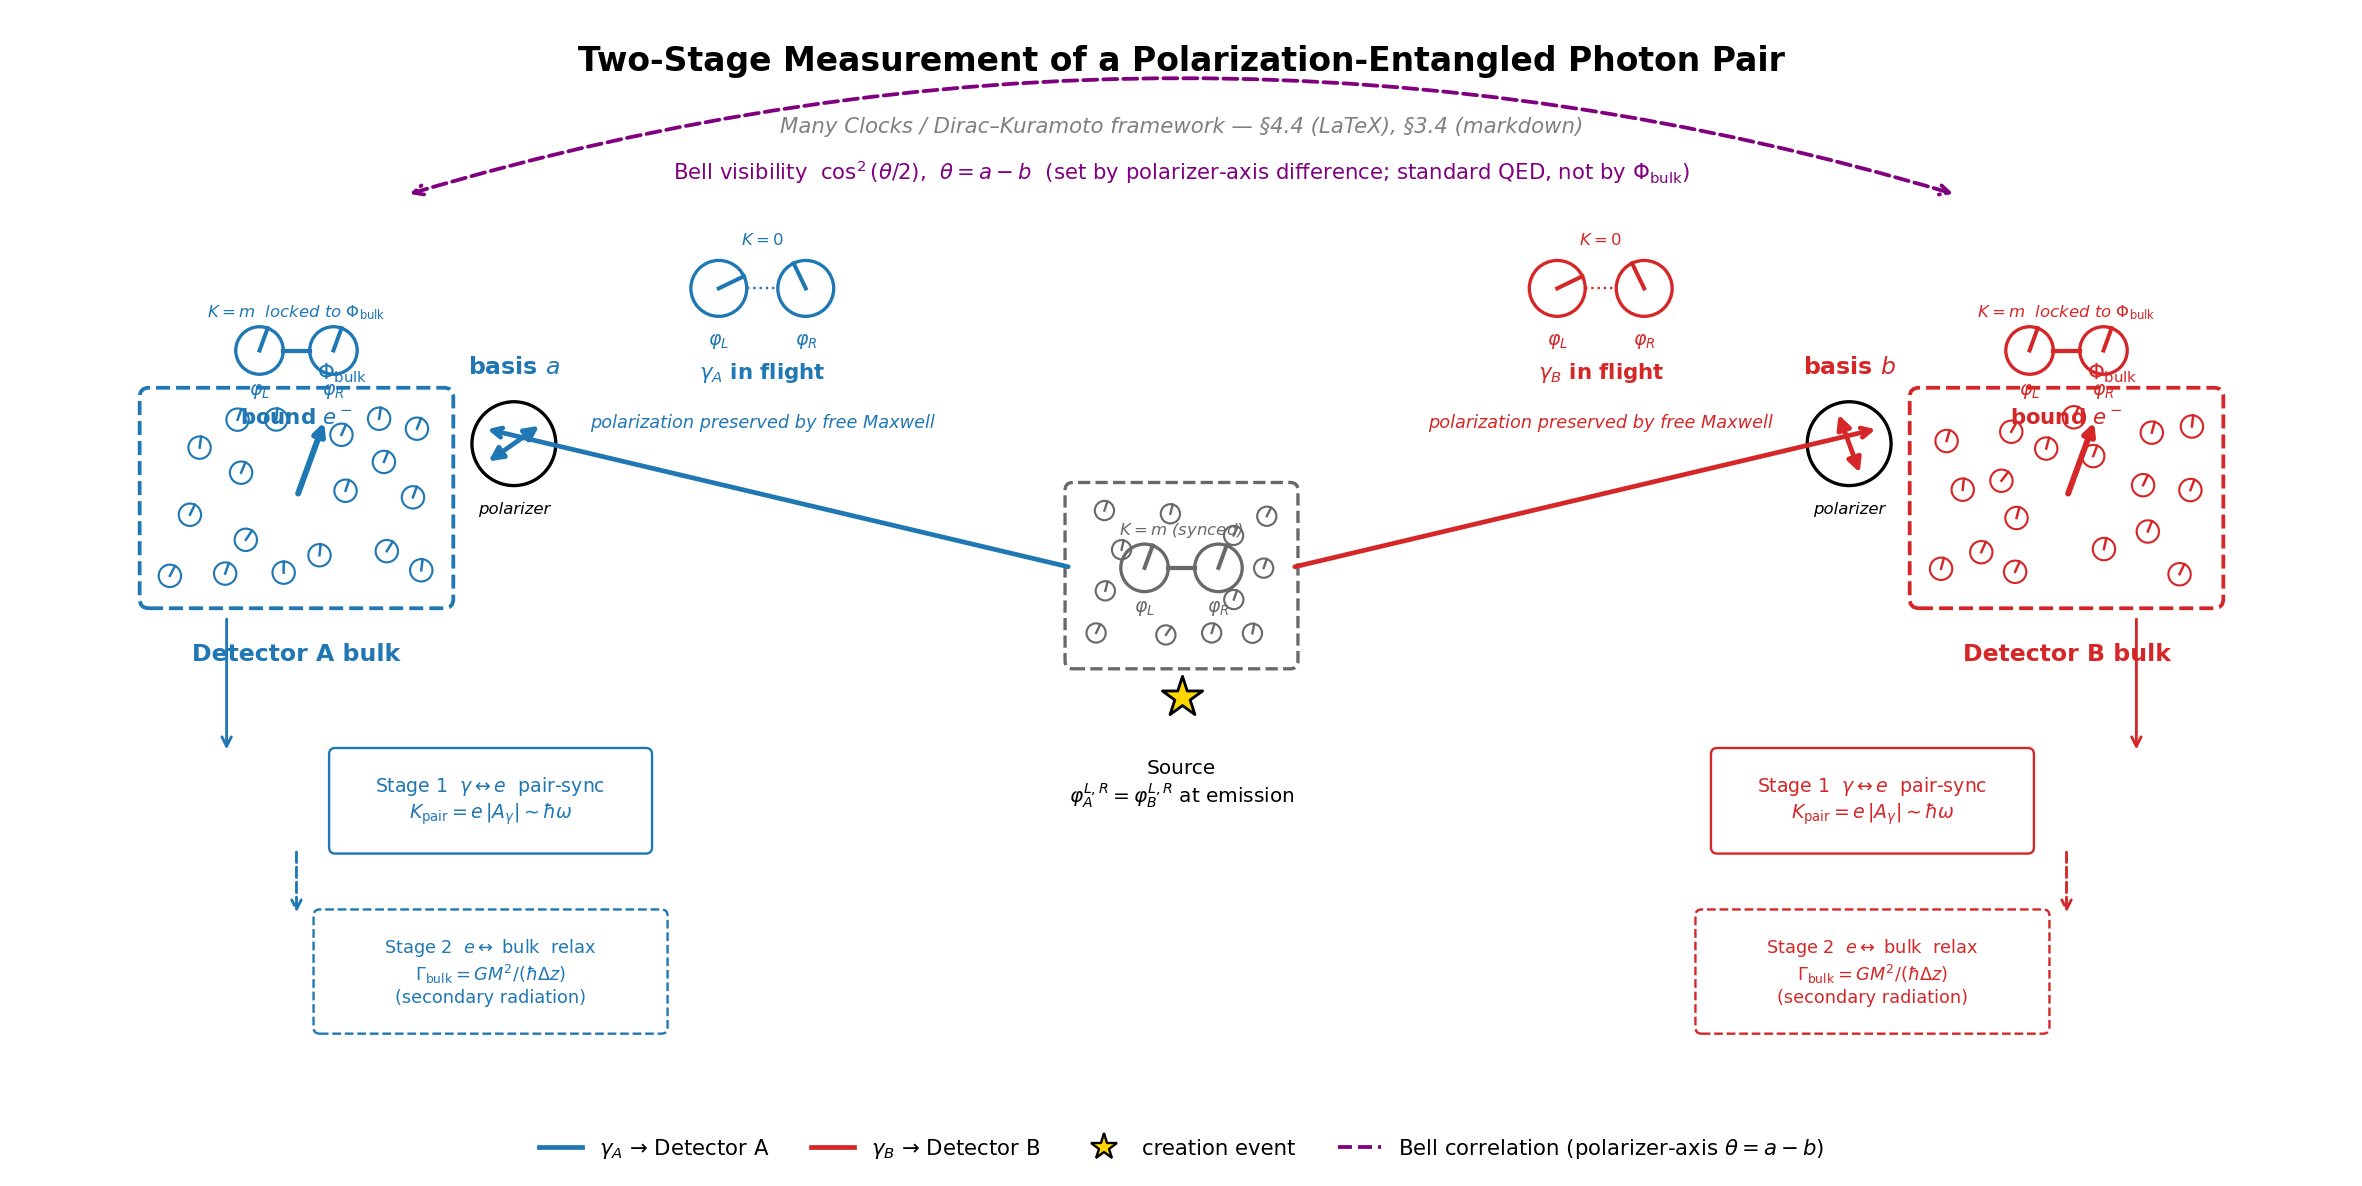
\includegraphics[width=\textwidth]{entangled_pair_two_stage.png}
\caption{Schematic of the two-stage measurement of a polarization-entangled
photon pair (not to scale). All three bulks (Source, Detector~A bulk,
Detector~B bulk) contain mini-clocks locked to a universal time-phase
$\Phi_{\mathrm{bulk}}$ ($\sim 70^\circ$ in the figure, with
$\sigma \approx 7^\circ$ jitter), reflecting environmental thermalization
across matter sharing a common gravitational potential. The entangled
photons $\gamma_A, \gamma_B$ carry matched chiral-clock phases at emission
but with $K = 0$ (dotted L--R link) and propagate freely between source
and detector. Each polarizer (black aperture with double-headed
transmission-axis arrow) defines an independently-set basis ($a$, $b$) on
the polarization Hilbert space---a separate degree of freedom from
$\Phi_{\mathrm{bulk}}$. At each detector, Stage~1 (solid box) is the
polarization projection onto the polarizer's transmitted-channel
eigenstate via pair-sync $K_{\mathrm{pair}}^{\gamma e}$ to a bound
electron; Stage~2 (dashed box) dissipates the projected state into the
bulk's $\Phi_{\mathrm{bulk}}$ via $\Gamma_{\mathrm{bulk}}$, releasing
secondary radiation. The $\cos^2(\theta/2)$ Bell visibility is set by the
polarizer-axis difference $\theta = a - b$ (standard QED), not by
$\Phi_{\mathrm{bulk}}$; the framework provides the physical mechanism for
the projection, not the statistics.}
\label{fig:two-stage}
\end{figure}

\paragraph{Stage 1 as polarization projection.} The $\cos^2(\theta/2)$
Bell visibility for photons is set by the polarizer-axis difference
$\theta = a - b$ acting on the photon's polarization Hilbert space---this
is standard QED, not a framework prediction (see \S 9.2). The framework's
contribution at Stage~1 is the \emph{physical mechanism} of projection:
the photon couples to a bulk-bound electron via $K_{\mathrm{pair}}^{\gamma e}$,
and the polarizer's macroscopic mechanical orientation determines which
transmitted-channel eigenstate the photon ends up in.
$\Phi_{\mathrm{bulk}}$, the bulk's collective time-phase, is a separate
quantity---approximately universal across the source and both detectors
when they share a similar gravitational environment, set by environmental
thermalization rather than by the polarizer geometry. The basis lives in
the polarizer's mechanical configuration; the time-phase lives in
$\Phi_{\mathrm{bulk}}$. Stage~1 connects the photon to the polarizer's
chosen basis; Stage~2 dissipates the resulting state's energy and phase
into $\Phi_{\mathrm{bulk}}$.

\paragraph{Why Stage 2 is automatic.} After the photon perturbs the
electron, $\phi_e$ is offset from $\Phi_{\mathrm{bulk}}$ by some
$\Delta\phi_e$. The mass-asymmetry argument of \S 4.3 applies directly:
the relaxation rate scales as
$\Gamma_{\mathrm{bulk}}\,(M_{\mathrm{bulk}}/m_e)$, overwhelmingly fast for
any macroscopic bulk. The energy released during this relaxation appears
as secondary radiation, partitioned by the size of the mismatch
$\hbar\dot\phi_e\,\Delta\phi_e$:
\begin{itemize}
\item below optical scale: virtual photon (Coulomb recoil) or phonon;
\item optical to $2m_e c^2$: real photon (fluorescence, bremsstrahlung);
\item $\geq 2m_e c^2$: $e^+e^-$ pair.
\end{itemize}

\paragraph{Gravitational dependence of the two stages.} Because the Bell
correlation is set by the polarizer-axis difference (standard QED) and
polarizer geometry is gravitationally invariant at leading order, the
visibility $\cos^2(\theta/2)$ is itself gravitationally invariant---
consistent with the agreement between Earth-bound and space-based Bell
tests. Gravity enters only at Stage~2, through
$\Gamma_{\mathrm{bulk}}$, with two subleading consequences. First, two
detectors at gravitational potentials $\Phi_A \neq \Phi_B$ have Stage-2
relaxation times that differ by $\Delta\Phi/c^2$, producing a correlated
timing offset between detection events that scales with the altitude split.
Second, if the gravitational potential difference along the photon paths
becomes large enough that the local bulk phases drift relative to each
other on the Stage-1 timescale $\tau_1 \sim 1/\omega$, a visibility floor
appears at order $\Delta\Phi/c^2$ per optical period---currently far below
experimental sensitivity but a clean target for satellite-to-ground
configurations. This locates the Penrose--Di\'osi mechanism unambiguously
at Stage~2: gravitational collapse acts on bulk relaxation, never on the
pair-sync that builds $\cos^2(\theta/2)$.

\paragraph{What this section does not yet pin down.}
\begin{enumerate}
\item The precise normalization of
  $\langle V_{\mathrm{int}}\rangle_{\mathrm{local}}$ (single-photon
  plane-wave vs.\ Compton-volume coherent state).
\item Whether the Stage~1/Stage~2 timing offset
  ($\tau_1 \sim 1/\omega$ vs.\ $\tau_2 \sim \hbar/E_{\mathrm{binding}}$)
  is empirically distinguishable from a single-event detection model.
\item Extension of
  $K_{\mathrm{pair}} = g_{\mathrm{int}}\langle V_{\mathrm{int}}\rangle$
  to weak and gluon-mediated pair interactions, where confinement and
  short-range structure complicate the local-amplitude reading.
\end{enumerate}

\subsection{Gravitational Coherence of the Bulk}

What maintains the coherence of the detector bulk itself? We propose that gravity
provides this role. The gravitational interaction between the ${\sim}10^{26}$ atoms in a
macroscopic detector provides a collective Kuramoto coupling that maintains a
common phase $\Phi_{\mathrm{bulk}}$ across the detector. This is analogous to the well-known
classical synchronization of metronomes on a shared massive platform.

\paragraph{Two senses of ``mass.''} A clarification is in order before writing
$\Gamma_{\mathrm{grav}}$. The mass $m$ appearing in the Kuramoto identification
$K = m$ of Section~2 is the Dirac mass of an \emph{elementary} fermion, generated
by the Higgs--Yukawa coupling $K = y_f v/\sqrt{2}$. The mass $M$ entering the
gravitational bulk coupling below is the \emph{total} gravitating mass-energy of
a composite body---for ordinary matter, ${\sim}99\%$ of which is QCD binding and
gluon-field energy in the nucleons, not Higgs-derived quark mass. The two are
different quantities entering at different scales: $K = m_{\mathrm{Higgs}}$
governs the L--R synchronization of a single spinor, while $\Gamma_{\mathrm{grav}}
\propto M_{\mathrm{total}}^2$ governs the pairwise gravitational synchronization
across the ${\sim}N^2/2$ constituents of a macroscopic detector. The bridge is the
equivalence principle: all forms of energy gravitate, so QCD binding contributes
to $\Gamma_{\mathrm{grav}}$ even though it does not contribute to the per-particle
Kuramoto coupling $K$.

The gravitational Kuramoto coupling for a mass $M$ interacting with a bulk at
distance $\Delta z$ is:
\begin{equation}
\Gamma_{\mathrm{grav}} = \frac{GM^2}{\hbar\,\Delta z}
\end{equation}
For macroscopic objects ($M \sim 1$~kg, $\Delta z \sim 1$~m), $\Gamma_{\mathrm{grav}} \sim 6 \times 10^{23}$~rad/s---an
extremely fast rate, which is precisely why bulk coherence is maintained so
effectively for macroscopic masses. The gravitational synchronization coupling
grows as $M^2$, ensuring that macroscopic objects are locked into collective phase
coherence far more strongly than microscopic particles.

\subsection{Connection to Penrose--Di\'osi}

This picture has a natural connection to Penrose's proposal~\cite{penrose1996} that
gravity causes quantum state reduction. Penrose argues that a superposition of
two mass configurations with different spacetime geometries is unstable, with
collapse timescale $\tau \sim \hbar/E_g$ where $E_g$ is the gravitational self-energy of the
superposition.

In the Kuramoto framework, this translates to: the gravitational bulk provides
a phase reference, and any quantum superposition that would require the particle
to maintain coherence against the gravitational synchronization pressure will
decohere on a timescale set by the gravitational coupling strength. The Penrose
energy $E_g$ maps onto the Kuramoto coupling rate $\Gamma_{\mathrm{grav}}$. Both
$E_g$ and $\Gamma_{\mathrm{grav}}$ are sourced by total gravitating mass-energy
(per the equivalence principle), so the correspondence is between physically
commensurable quantities rather than an artifact of notation. The two frameworks
predict the same qualitative behavior---heavier objects decohere faster---from
different dynamical starting points.

\subsection{Geometric Picture: The Coherence Sub-Manifold}

The synchronization, interference, and measurement processes described above admit
a unified geometric reading. Each Kuramoto phase oscillator carries a phase
$\phi \in S^1$, so the joint state of $N$ oscillators lives on the $N$-torus
$T^N = (S^1)^N$. There are not separate manifolds for separate systems; there is
one product space whose factors index the oscillators.

Within this product space, every lock condition picks out a lower-dimensional
sub-manifold:

\begin{itemize}
\item For a single Dirac spinor, the L--R lock $\phi_L - \phi_R = \delta_{CP}$
  defines a $1$-dimensional curve inside $T^2_{\mathrm{spinor}}$.
\item For the detector bulk, the alignment condition
  $\phi_1 = \phi_2 = \cdots = \phi_N = \Phi_{\mathrm{bulk}}$ defines a
  $1$-dimensional diagonal circle inside $T^N_{\mathrm{bulk}}$.
\item For a measured particle, the coupling condition $\phi_A = \Phi_{\mathrm{bulk}}$
  defines a sub-manifold inside the joint particle--detector space
  $T^2_{\mathrm{particle}} \times T^N_{\mathrm{bulk}}$.
\end{itemize}

The post-measurement state lies in the \emph{intersection} of these sub-manifolds.
The dimensional collapse is dramatic: from ${\sim}10^{26}$ free phase coordinates
down to effectively one global locked phase.

We refer to this intersection as the \textbf{coherence sub-manifold}, because it
plays two complementary roles simultaneously:

\begin{enumerate}
\item \textbf{Dynamical role (attractor).} It is the locus toward which Kuramoto
  trajectories asymptote. Off the coherence sub-manifold, oscillator phases drift
  relative to one another; on it, the lock relations are stationary.
\item \textbf{Observational role (interference locus).} It is the locus on which
  coherent phase relations are well-defined. Off the sub-manifold, relative phases
  $\Delta\phi$ wander ergodically over $S^1$ and any interference term
  $\cos(\Delta\phi)$ averages to zero; on it, $\Delta\phi$ is pinned and
  interference is sharp and observable. The Bell correlation $\cos(2\theta)$ of
  Section~3 is, geometrically, a function evaluated on the locked sub-manifold of
  the two-particle phase space---it is well-defined only there.
\end{enumerate}

This dual role yields a useful re-statement of measurement in geometric terms:
\emph{the measurement event is not the destruction of interference but the
re-routing of the joint trajectory from one coherence sub-manifold to another.}
The particle leaves the entanglement sub-manifold (where it shared coherence with
its partner) and joins the bulk sub-manifold (where it shares coherence with the
detector). What standard accounts call ``decoherence'' is, in this picture, a
change of which sub-manifold the joint state lives on, not a loss of coherent
structure as such.

\subsection{What This Section Does Not Claim}

The re-synchronization picture is interpretive. It does not:

\begin{enumerate}
\item Derive decoherence rates quantitatively from Kuramoto parameters (this would
  require a full quantum treatment of many-body Kuramoto dynamics)
\item The Born rule probability $P = |\alpha|^2$ is addressed in Section~6
\item Provide a Lorentz-covariant formulation of the measurement process
\end{enumerate}

%% ============================================================
\section{Single-World Energy Accounting}

\subsection{The Energy Bookkeeping Problem}

Before measurement, a system $\psi = \alpha|0\rangle + \beta|1\rangle$ carries total energy $E = \hbar\omega$. After
measurement produces outcome $|0\rangle$, what happens to the energy associated with the
$|\beta|^2$ amplitude?

\begin{itemize}
\item Copenhagen: it vanishes---the wavefunction collapses
\item Everett: it persists in an inaccessible branch
\item Bohmian: the pilot wave carries no energy
\end{itemize}

Each answer is unsatisfying. We propose a fourth:

\subsection{Thermalization of Residual Amplitude}

In the Kuramoto measurement process (Section~4), the detector resonantly absorbs
the energy quantum $\hbar\omega_0$ corresponding to the realized outcome. The residual
amplitude---the portion of the wavefunction that did not synchronize with the
detector---has no resonant absorber available.

We propose that this residual couples weakly to the broadband electromagnetic
environment and thermalizes as low-frequency radiation:
\begin{equation}
E_{\mathrm{residual}} = (1 - P) \cdot \hbar\omega
\end{equation}
where $P = |\alpha|^2$ is the Born-rule probability of the realized outcome.

\subsection{A Single World}

This gives a definite single-world account:

\begin{enumerate}
\item $\psi$ is a real physical field carrying energy
\item Measurement is resonant energy extraction (the detector takes $\hbar\omega_0$)
\item The residual thermalizes into the vacuum
\item One classical fact results, with Born-rule probability
\item No branch is created; the residual energy is in this world as thermal radiation
\end{enumerate}

\subsection{Honest Caveats}

This proposal is the most speculative part of the paper:

\begin{enumerate}
\item The thermalization rate is not derived from first principles
\item The mechanism by which residual amplitude ``finds'' the thermal bath is not
  specified beyond analogy with spontaneous emission
\item The Born rule is derived from synchronization statistics (Section~6)
\item We do not claim this resolves the measurement problem---it provides a physical
  picture that is more complete than Copenhagen's ``collapse'' but not yet a
  rigorous derivation
\end{enumerate}

\textbf{What we explicitly do not claim:} We previously explored whether accumulated
thermal residuals could account for the observed dark energy density. While a
crude order-of-magnitude estimate was suggestive, detailed analysis revealed the
calculation to be unreliable, and we withdraw this as a prediction. The
thermalization proposal stands independently of any cosmological implications.

%% ============================================================
\section{The Born Rule from Synchronization Statistics}

\subsection{The Problem}

The Born rule---$P = |\psi|^2$---is the bridge between the mathematical formalism and
experimental outcomes. In standard quantum mechanics it is postulated, not derived.
Copenhagen asserts it. Everett's many-worlds claims to derive it from branch
counting, but this remains contested. The measurement problem, at its core, is the
question of why probability equals the squared modulus of a complex amplitude.

\subsection{The Kuramoto Order Parameter}

The Kuramoto model provides a natural answer. For $N$ coupled oscillators with
phases $\phi_1, \phi_2, \ldots, \phi_N$, the degree of collective synchronization is measured by
the order parameter:
\begin{equation}
R \cdot e^{i\Psi} = \frac{1}{N}\sum_{j=1}^{N} e^{i\phi_j} \tag{8}
\end{equation}
where $R \in [0,1]$ is the synchronization amplitude and $\Psi$ is the collective phase.
The probability that a single oscillator with phase $\phi$ locks to the collective
is proportional to $R^2$---the squared modulus of the complex order parameter.

This is not a coincidence. It is a general property of phase-coupled oscillator
systems: the coupling efficiency between a single oscillator and a synchronized
cluster depends on the squared amplitude of the cluster's complex coherence.

\subsection{Application to Quantum Measurement}

Consider a particle in superposition $\psi = \alpha|0\rangle + \beta|1\rangle$ arriving at a detector.
The detector is a macroscopic Kuramoto-synchronized bulk with $N \gg 1$ oscillators
locked to phase $\Phi_{\mathrm{bulk}}$.

The particle carries two components, each a complex amplitude with a definite phase:

\begin{itemize}
\item Component $|0\rangle$ with amplitude $\alpha = |\alpha|e^{i\phi_0}$
\item Component $|1\rangle$ with amplitude $\beta = |\beta|e^{i\phi_1}$
\end{itemize}

The Kuramoto synchronization process couples the particle to the detector bulk.
The coupling strength between the particle component and the detector depends on
the complex overlap---the projection of the particle's phase oscillator onto
the detector's synchronized state.

For a complex oscillator with amplitude $A \cdot e^{i\phi}$ coupling to a reference
oscillator, the synchronization probability is:
\begin{equation}
P_{\mathrm{sync}} \propto |A \cdot e^{i\phi}|^2 = |A|^2 \tag{9}
\end{equation}
The phase determines \emph{which} detector eigenstate is reached. The amplitude
determines \emph{how likely} that synchronization is. Averaging over the random bulk
phase $\Phi_{\mathrm{bulk}}$ (which is uniformly distributed over $[0, 2\pi)$ from the particle's
perspective), all cross terms vanish:
\begin{equation}
\langle e^{i(\phi_0 - \phi_1)} \rangle_{\Phi_{\mathrm{bulk}}} = 0 \tag{10}
\end{equation}
Only the diagonal terms survive:
\begin{equation}
P(|0\rangle) = |\alpha|^2, \qquad P(|1\rangle) = |\beta|^2 \tag{11}
\end{equation}
This is the Born rule, derived from Kuramoto synchronization statistics rather
than postulated.

\subsection{Why the Squared Modulus?}

The answer is geometric. The wave function is complex because the internal clock
is a phase oscillator---it lives on a circle in the complex plane. The probability
of synchronization between two oscillators is the squared modulus of their complex
overlap because:

\begin{enumerate}
\item The coupling is linear in the complex amplitude (Kuramoto sine coupling)
\item Probability is quadratic in the coupling (energy transfer $\propto$ amplitude$^2$)
\item The complex phase averages out over the bulk, leaving only $|\text{amplitude}|^2$
\end{enumerate}

This is identical to why the intensity of a classical wave is proportional to the
squared amplitude---and it should be, because the wave function \emph{is} a real
oscillating field in this framework. The Born rule is the statement that quantum
probability equals wave intensity, which is the natural measure for any physical
wave coupling to a detector.

\subsection{Connection to the Zero-Point Floor}

The zero-point phase noise $\sigma_\phi(0) = 1/\sqrt{2}$~rad (Section~9 of the equations
reference) sets a minimum uncertainty in the synchronization process. Even at
$T = 0$, a particle cannot synchronize with perfect fidelity---the irreducible
phase noise means that the probability $|\alpha|^2$ always has a minimum variance.
This connects the Born rule to the Heisenberg uncertainty principle: both
emerge from the same zero-point phase floor.

\subsection{What This Derivation Requires}

The derivation rests on three assumptions, all already present in the framework:

\begin{enumerate}
\item The wave function is a physical oscillating field (not merely a calculational tool)
\item Measurement is Kuramoto synchronization to a macroscopic bulk
\item The detector's bulk phase is uniformly distributed relative to the particle's phase basis
\end{enumerate}

Assumption~3 is the most important. It is equivalent to the statement that the
detector has no prior knowledge of which outcome will occur---it is the
Kuramoto equivalent of the assumption of measurement independence in Bell's
theorem. The detector synchronizes to whichever component has the largest
coupling amplitude, with probability proportional to $|\text{amplitude}|^2$.

%% ============================================================
\section{Zitterbewegung as a Beat Frequency}

Zitterbewegung~\cite{schrodinger1930}---the rapid oscillatory motion of a Dirac electron at frequency
$2mc^2/\hbar$---is conventionally attributed to interference between positive and negative
frequency components. In the phase-clock picture, it has a more intuitive
interpretation.

The temporal clock oscillates at $\omega_t = E/\hbar$. The spatial clock oscillates at
$\omega_s = p^2/(m\gamma\cdot\hbar)$. Their beat frequency in the non-relativistic limit:
\begin{equation}
\omega_{\mathrm{Zitter}} \approx \frac{2mc^2}{\hbar} \tag{12}
\end{equation}
This is exactly the known Zitterbewegung frequency. In the phase-clock
interpretation, Zitterbewegung is the \textbf{beat note between the temporal and spatial
clocks}---observable whenever the two clocks are not perfectly synchronized.

When $K = m$ is large (heavy particle), synchronization is fast and the beat has
small amplitude. When $K$ is small (light particle), the clocks are loosely coupled
and the beat has larger amplitude. A massless particle ($K = 0$) has permanently
unsynchronized clocks at $\theta_{\mathrm{rel}} = 90^\circ$ and no Zitterbewegung---consistent with
photons.

%% ============================================================
\section{Antiparticles and CP Violation}

\subsection{Antiparticles as Time-Reversed Clocks}

The negative-energy Dirac solution $v(p,s)e^{+iEt/\hbar}$ has temporal phase running
in the opposite sense to a positive-energy particle. In the Kuramoto framework:
\textbf{antiparticles are particles with time-reversed phase clocks} ($\phi \to -\phi$).

This is not a reinterpretation---it is already implicit in the Feynman--St\"uckelberg
interpretation~\cite{stueckelberg1941,feynman1949}. The phase-clock language makes it explicit.

\subsection{CP Violation as Synchronization Asymmetry}

The Kuramoto equations (2a, 2b) contain the CP-violating phase $\delta_{CP}$. For
particles, the equilibrium phase lock is $\Delta\phi = +\delta_{CP}$; for antiparticles,
$\Delta\phi = -\delta_{CP}$.

When particle and antiparticle meet for annihilation, their synchronization
efficiency depends on the phase mismatch:
\begin{equation}
\sigma_{\mathrm{ann}} \propto |\langle\psi_{\mathrm{particle}}|\psi_{\mathrm{antiparticle}}\rangle|^2
\propto 1 + \varepsilon\cos(\delta_{CP})
\end{equation}
The small asymmetry $\varepsilon$ accumulates over the early universe to produce the observed
baryon asymmetry $\eta \sim 10^{-9}$. This is a qualitative mechanism, not a quantitative
prediction---a full calculation requires electroweak baryogenesis beyond the scope
of this paper.

%% ============================================================
\section{Extension to Photons via the Riemann--Silberstein Form}

Photons are not Dirac particles. They are spin-1 vector bosons described by
Maxwell's equations, with no rest mass to couple chiral sectors. The
framework's central identification $K = m$ therefore does not apply directly:
there is no mass term to set a Kuramoto coupling between photon helicities.
We address this by separating two questions that earlier formulations
conflated: (i)~where do photon Bell correlations come from? and (ii)~where
does the framework's measurement mechanism enter for photons?

\subsection{The Riemann--Silberstein Form of Maxwell}

Maxwell's free equations can be written in a Weyl-like first-order form
using the Riemann--Silberstein vector:
\begin{equation}
\mathbf{F} = \mathbf{E} + i\,\mathbf{B}, \qquad
i\,\partial_t \mathbf{F} = c\,\nabla \times \mathbf{F}, \qquad
\nabla \cdot \mathbf{F} = 0
\end{equation}
The two helicity eigenstates $\mathbf{F}_+$ and $\mathbf{F}_-$ (right- and
left-circular polarizations) are independent---there is no mass term, and
the structure mirrors the $m = 0$ chiral limit of the Dirac equation: two
decoupled clocks, $\theta_{\mathrm{rel}} = \pi/2$ permanently. A Kuramoto
coupling between $\mathbf{F}_+$ and $\mathbf{F}_-$ of a single photon is
identically zero in vacuum.

\subsection{Where Photon Bell Correlations Come From}

The polarization Hilbert space of a photon is two-dimensional, spanned by
any orthogonal pair (H/V, $\pm$, L/R). It is mathematically isomorphic to
the spin-$\tfrac{1}{2}$ Hilbert space, with the Poincar\'e sphere playing
the role of the Bloch sphere. For two polarization-entangled photons in
the singlet state, the standard quantum correlation is
\begin{equation}
E_\gamma(a, b) = -\cos\!\bigl(2(a-b)\bigr)
\end{equation}
and the CHSH bound saturates at $2\sqrt{2}$. The factor of 2 in the angular
dependence reflects the $\pi$-periodicity of polarizers (vs.\ $2\pi$
-periodicity of Stern--Gerlach analyzers).

This correlation is a property of the polarization Hilbert space, not of
any chiral coupling. It is delivered by standard QED---the same way
standard QM with the Dirac spinor delivers the $-\cos(a-b)$ correlation
for spin-$\tfrac{1}{2}$ pairs (Section~2). In both cases, the framework
does not derive the Bell correlations; the underlying Hilbert-space
structure does. The framework's contribution lies elsewhere.

\subsection{The Measurement Mechanism Transfers to Photons}

The framework's central interpretive claim---measurement is Kuramoto
re-synchronization to the detector bulk (Section~4)---does not depend on
the $K = m$ identification for its physical content. It requires only that
the system being measured carries a phase clock that can be synchronized
to the detector. Photons satisfy this: each polarization mode carries a
definite phase, and at detection the photon's polarization clock locks to
the polarizer's selected channel (transmitted vs.\ rejected).

The Kuramoto coupling for the photon--detector interaction is not zero---it
is set by the photon's interaction with the detector matter (typically
dipole coupling $-\mathbf{d}\cdot\mathbf{E}$), not by any vacuum mass term.
For a photon of energy $E = \hbar\omega$ coupling to a near-resonant
detector channel, the natural Kuramoto rate scales with the photon's own
oscillation frequency:
\begin{equation}
K_\gamma \sim \omega = \frac{E}{\hbar}, \qquad
\tau_{\mathrm{sync}} \sim \frac{1}{K_\gamma} = \frac{\hbar}{E} \tag{13}
\end{equation}
A 2~eV optical photon synchronizes to its detector in ${\sim}0.3$~fs; a
10~keV X-ray locks in ${\sim}10^{-19}$~s. Higher-energy photons
synchronize faster---the Kuramoto rate is set by the photon's energy via
its interaction with the detector, rather than by any rest mass.

This is the photon analog of $K = m$ for fermions: in both cases, the
synchronization rate to the detector is set by the energy scale that
characterizes the system's coupling to its environment. For massive
fermions at rest that scale is $mc^2$ (the Compton frequency); for photons
it is $\hbar\omega$ (the photon's own frequency).

\subsection{Gravitational Decoherence and the Linewidth-Dependent Bell Test}

Two photon time scales must be kept distinct:
\begin{itemize}
\item $\tau_{\mathrm{sync}} = \hbar/E$---the time for Kuramoto re-sync to
  the detector to complete (set by photon energy);
\item $\tau_{\mathrm{coh}} = 1/\Delta\nu$---the photon's coherence time
  during measurement (set by \emph{linewidth}, independent of central
  energy).
\end{itemize}

For a given measurement event, the photon is in coherent superposition
during the $\tau_{\mathrm{coh}}$ window. If the two detectors A and B in a
Bell test are at different gravitational potentials, their bulk phases
$\Phi_{\mathrm{bulk}}(A)$ and $\Phi_{\mathrm{bulk}}(B)$ accumulate a
relative offset proportional to
$\omega \cdot \Delta\Phi_{\mathrm{grav}}/c^2 \cdot \tau_{\mathrm{coh}}$.
When this offset exceeds ${\sim}1$~rad, the singlet correlation degrades.

This is the linewidth-dependent gravitational Bell prediction
(\texttt{predictions.py} P6b), in self-consistent form:
\begin{equation}
\delta\phi_{\mathrm{grav}} = \omega \cdot \frac{\Delta\Phi_{\mathrm{grav}}}{c^2}
\cdot \tau_{\mathrm{coh}}
= \frac{\omega \cdot \Delta\Phi_{\mathrm{grav}}}{c^2 \cdot \Delta\nu} \tag{14}
\end{equation}
\begin{equation}
\mathrm{CHSH}(\Delta\nu) = 2\sqrt{2} \cdot
\exp\!\left(-\frac{\delta\phi_{\mathrm{grav}}^2}{2}\right) \tag{15}
\end{equation}

Standard QM/QED predicts CHSH is independent of photon linewidth at fixed
entanglement fidelity. The framework predicts it decreases with narrowing
linewidth in the presence of a gravitational potential difference between
the detectors. Tests are in reach using cavity-filtered narrow-linewidth
photons at altitude differences of a few km (terrestrial) or with
Earth--satellite baselines.

The discriminating measurement is the joint linewidth $\times$ altitude
scan with narrow-linewidth photons; photon energy is one knob among three
(along with linewidth $\Delta\nu$ and altitude split
$\Delta\Phi_{\mathrm{grav}}$), not a discriminator on its own.

\subsection{Photons and Penrose Objective Reduction}

The gravitational synchronization rate
$\Gamma_{\mathrm{grav}} = GM^2/(\hbar\Delta z)$ (Section~4.5) vanishes
identically for a massless particle. Equivalently, the Penrose
objective-reduction timescale $\tau_{\mathrm{OR}} = \pi\hbar/E_G$ with
$E_G = Gm^2/\Delta x$ becomes infinite for $m = 0$. \textbf{The
gravitational classicalization channel that drives massive systems toward
definite outcomes is silent for photons.}

This matches Penrose's own position. The OR proposal is designed for
superpositions of macroscopically distinct \emph{mass} configurations
(mirrors, mesoscopic test masses); Penrose has been explicit that single
photons fall outside its remit because they have no rest mass to source
the gravitational self-energy.

In the framework's reading, a photon therefore has only two pathways into
the classical domain:
\begin{enumerate}
\item \textbf{Measurement (active).} Kuramoto re-synchronization to a
  quantized detector channel (\S 9.3). A single photon hitting a
  photodetector produces a definite click; this is the only mechanism by
  which an isolated photon classicalizes.
\item \textbf{Coherent-state averaging (many-photon).} A macroscopically
  populated mode (laser light, classical EM) has a positive Wigner
  function and obeys Maxwell's equations classically. The classical limit
  emerges through statistical superposition of many photon modes, not
  through any internal collapse mechanism.
\end{enumerate}

A single photon in vacuum, between emission and detection, is
\textbf{perpetually quantum}---it does not gravitationally classicalize,
and it has no way to do so internally. This is consistent with the
experimental fact that single-photon Bell tests preserve full coherence
over kilometer-scale separations and Earth--satellite baselines, where any
internal classicalization mechanism would have produced observable
degradation.

One subtlety: photons do follow null geodesics in curved spacetime
(gravitational lensing, Shapiro delay). This is unitary classical
evolution of the photon's trajectory, not collapse or decoherence of its
quantum state---it bends paths without classicalizing states.

The silence of the gravitational channel for photons is consistent with
the linewidth-dependent prediction in \S 9.4, which attributes the
gravitational effect not to the photon in flight but to the bulk-phase
mismatch between detectors A and B at different gravitational potentials.
The photon is the messenger; the gravitational decoherence is in the
detectors.

\subsection{What Remains Open}

Two questions are not resolved by this section:
\begin{enumerate}
\item \textbf{A first-principles derivation of $K_\gamma$ from QED.} We
  have asserted $K_\gamma \sim \omega$ as the natural scaling, motivated
  by photon--detector dipole coupling. A rigorous derivation would relate
  $K_\gamma$ to the absorption matrix element
  $\langle e|\mathbf{d}|g\rangle$ for the specific detector channel and
  compute the actual sync time for realistic photodetectors
  (photomultipliers, avalanche photodiodes, superconducting nanowire
  detectors).
\item \textbf{The microscopic mechanism for the discrete click.}
  Section~6 attributes discrete clicks to the threshold structure of
  detector channels. For photons, this corresponds to the photoelectric
  or photon-counting threshold of the detection element. The framework
  provides a mechanism (re-sync to a quantized channel) but does not yet
  derive the threshold from first principles.
\end{enumerate}

These are tractable extensions, not framework contradictions. The
photon-coupling problem---flagged in earlier drafts as the framework's
most serious open question---reduces to a pair of well-defined technical
issues once the Bell correlations are correctly attributed to the
polarization Hilbert space rather than to any Kuramoto coupling between
photon helicities.

%% ============================================================
\section{Qualitative Predictions and Consistency Checks}

We distinguish between predictions that follow from the mathematical identification
(Section~2) and those that follow from the interpretive claims (Sections~4--6).

\subsection{From the Mathematical Identification}

\textbf{P1---Three-term decomposition of Bell correlations.} For massive entangled
particles, the correlation $E(a,b) = -\cos(a-b)$ decomposes into $E_{LL} + E_{SS} + E_{LS}$,
with the relative contributions depending on $\theta_{\mathrm{rel}} = \arcsin(v/c)$. While $E_{\mathrm{total}}$
is Lorentz-invariant, the decomposition itself is new and numerically verified.
A hypothetical experiment separately addressing large and small spinor components
could reveal this structure.

\textbf{P2---Zitterbewegung as clock beat.} The identification of $\omega_{\mathrm{Zitter}} = 2mc^2/\hbar$
as the beat frequency between temporal and spatial clocks is consistent with all
known properties of Zitterbewegung. Trapped-ion simulations with tunable effective
mass~\cite{gerritsma2010} could probe the transition from locked to unlocked
clock behavior as effective mass passes through zero.

\subsection{From the Interpretive Framework}

\textbf{P3---Decoherence rate scaling with mass.} If the Kuramoto synchronization rate
is $K = m$, heavier particles should decohere faster: $\tau_{\mathrm{sync}} \sim \hbar/m$. This is
qualitatively consistent with the observation that macroscopic objects exhibit
essentially instantaneous decoherence while electrons maintain quantum coherence
over longer timescales. A precision measurement of decoherence rate as a function
of particle mass (electrons, muons, pions, kaons) could test whether
$\tau_{\mathrm{decoherence}} \propto 1/m$.

\textbf{P4---Higgs coupling and synchronization rate.} If $K = y_f \cdot \langle\phi\rangle = m$, then
decoherence rates for entangled fermion pairs should scale linearly with mass.
Comparing entanglement decay times for kaon pairs ($m_K = 494$~MeV) versus B-meson
pairs ($m_B = 5{,}280$~MeV) should show $\tau_B/\tau_K \sim m_K/m_B \approx 0.094$. Existing
collider data on neutral kaon and B-meson decoherence could be analyzed.

\textbf{P5---Gravitationally-weighted secondary-radiation rate.} The Stage~2
bulk relaxation (\S 4.4) emits secondary radiation (virtual photon, real
photon, or $e^+e^-$ pair, depending on the energy mismatch) at a rate set
by $\Gamma_{\mathrm{bulk}}$. Because $\Gamma_{\mathrm{bulk}}$ depends on
the local mass--energy distribution and is therefore subject to
gravitational redshift, the secondary-emission rate during a detection
event scales as $1 + \Phi_{\mathrm{grav}}/c^2$ at leading order. Two
detectors at different gravitational potentials should register a
fractional rate difference of order $\Delta\Phi/c^2$---roughly $10^{-13}$
for a 1000~km altitude split. This is below current sensitivity but a
clean signature unique to the two-stage framework: neither standard
decoherence theory nor Penrose--Di\'osi predicts gravity-dependent timing
of detection-induced secondary emission.

\subsection{Honest Assessment}

These predictions are qualitative scaling arguments, not quantitative predictions
with computed coefficients. The framework in its current form is an interpretation
---it provides a physical mechanism consistent with known decoherence behavior but
does not yet make predictions distinguishable from standard decoherence theory.
This is the main limitation and the main avenue for future work.

%% ============================================================
\section{Comparison with Existing Frameworks}

\subsection{Interpretations of Quantum Mechanics}

\begin{table}[H]
\centering
\small
\begin{tabular}{p{2.2cm}p{1.5cm}p{1.5cm}p{1.5cm}p{1.7cm}p{1.7cm}p{2cm}}
\toprule
\textbf{Property} & \textbf{Copen\-hagen} & \textbf{Everett MWI} & \textbf{Bohmian} & \textbf{GRW/CSL}~\cite{grw1986,pearle1989} & \textbf{Super\-determinism} & \textbf{This work} \\
\midrule
$\psi$ is real? & No & Yes & Yes & Yes & Varies & \textbf{Yes} \\
Collapse? & Postulated & No & No & Stochastic & Not needed & \textbf{Re-sync} \\
Branching? & No & Yes ($\infty$) & No & No & No & \textbf{No} \\
Residual energy? & Discarded & In branches & Pilot wave & Noise & Not addressed & \textbf{Thermal vacuum} \\
Single world? & By fiat & No & Yes & Yes & Yes & \textbf{Yes (physics)} \\
Mechanism? & None & None & Pilot wave & Random hits & Initial cond. & \textbf{Kuramoto sync} \\
Bell? & Accepted & Accepted & Accepted (NL) & Accepted & Denied & \textbf{Accepted} \\
Born rule & Postulated & Derived? & Derived & Modified & Derived? & \textbf{Derived (\S6)} \\
\bottomrule
\end{tabular}
\end{table}

\subsection{Decoherence Models}

The closest existing framework is the Penrose--Di\'osi gravitational decoherence
model~\cite{penrose1996,diosi1989}. Both that model and ours identify gravity as
the agent of classicalization. The key differences:

\begin{itemize}
\item Penrose--Di\'osi: collapse timescale $\tau \sim \hbar/E_g$ (gravitational self-energy)
\item This work: decoherence timescale set by Kuramoto re-synchronization rate to
  the gravitational bulk
\end{itemize}

The predictions are qualitatively similar (heavier $\to$ faster decoherence) but
derive from different dynamics. A quantitative comparison awaits a full
derivation of Kuramoto decoherence rates from first principles.

\subsection{Zurek's Einselection}

Zurek's quantum Darwinism~\cite{zurek2003,zurek2009} identifies ``pointer states'' as
states that survive interaction with the environment. In the Kuramoto picture,
pointer states are the synchronized states---the phase-locked configurations
that are stable under coupling to the macroscopic bulk. States that cannot
synchronize (superpositions of macroscopically distinct mass configurations)
are dynamically unstable and decohere. This is consistent with einselection
but provides a specific dynamical mechanism (phase locking) for why certain
states survive.

\subsection{Superdeterminism}

Superdeterminism~\cite{thooft2016,bell1976} escapes Bell's theorem by denying
measurement independence: the hidden variable $\lambda$ and the detector settings $(a, b)$
are correlated because they share a common causal past. If $\rho(\lambda|a,b) \neq \rho(\lambda)$,
Bell's derivation does not go through, and local hidden variable models can
reproduce quantum correlations.

This comparison is important because the measurement-independence loophole through
the gravitational bulk phase $\Phi_{\mathrm{bulk}}$---arguing that since both detectors and the
particle source share a common gravitational field, their states are
correlated---might seem to apply here. We explicitly reject this route in the
present paper, as discussed below.

\textbf{Why this framework is not superdeterministic:}

\begin{enumerate}
\item \textbf{We do not challenge Bell's theorem.} The quantum correlations
  $E(a,b) = -\cos(a-b)$ are accepted as arising from the entangled singlet state
  and the full Dirac spinor structure---standard quantum mechanics. No hidden
  variable model is proposed to replace them.

\item \textbf{Measurement independence is preserved.} The experimenter's choice of
  detector angle is not constrained by the framework. The gravitational bulk
  phase $\Phi_{\mathrm{bulk}}$ maintains detector coherence (Section~4.4) but does not
  determine or correlate with measurement settings.

\item \textbf{The role of gravity is different.} In superdeterminism, correlations
  between $\lambda$ and $(a,b)$ must be fine-tuned to reproduce quantum predictions
  exactly---a conspiracy that many physicists find unacceptable. In this framework, gravity provides the
  synchronization bath for the \emph{measurement process} (decoherence), not for the
  \emph{correlations} (which are quantum mechanical).

\item \textbf{No retrocausality or conspiracy.} Superdeterministic models require that
  the state of the universe at the Big Bang already encodes which detector
  settings will be chosen in a 2015 Bell test~\cite{aspect1982}. This framework requires only
  that macroscopic detectors are phase-coherent objects immersed in a
  gravitational field---a physically uncontroversial claim.
\end{enumerate}

The distinction can be stated concisely: superdeterminism says the correlations
are classical but hidden in the initial conditions. This framework says the
correlations are quantum, and the Kuramoto mechanism explains how they are
\emph{revealed} (measurement) and \emph{degraded} (decoherence), not how they are
\emph{produced}.

%% ============================================================
\section{Discussion}

\subsection{The Interpretive Status}

This paper presents a mathematical identification (Dirac = Kuramoto) and an
interpretive framework built on it (measurement = re-synchronization). The
mathematical identification is verifiable and, we believe, novel. The
interpretive framework is physically motivated but not yet quantitatively
predictive beyond standard decoherence.

We are in the category of interpretation papers---alongside many-worlds,
Bohmian mechanics, and relational QM~\cite{rovelli1996}. The contribution is not new equations
but a new way of reading existing equations that provides physical intuition
for the measurement process.

\subsection{The Historical Note}

The timeline is suggestive:

\begin{itemize}
\item 1928: Dirac equation (the two-clock structure)
\item 1935: EPR paper~\cite{epr1935} (``spooky action at a distance'')
\item 1964: Bell's theorem
\item 1975: Kuramoto model
\end{itemize}

The relativistic spinor structure that produces the full quantum correlation
existed 36 years before Bell showed it was needed. The synchronization framework
that describes the coupling existed 11 years after Bell. The identification
presented here connects these threads.

\subsection{Future Directions}

Three directions could elevate this from interpretation to testable theory:

\begin{enumerate}
\item \textbf{Quantitative decoherence rates.} Derive decoherence timescales from
  Kuramoto parameters in a many-body quantum setting. If these reproduce known
  rates for specific systems (e.g., superconducting qubits, trapped ions), the
  framework gains predictive power. If they differ, the framework makes testable
  predictions.

\item \textbf{Born rule---rigorous proof.} Section~6 argues that $P = |\alpha|^2$ follows from
  Kuramoto synchronization statistics: the squared modulus of the complex
  coupling amplitude determines synchronization probability, and averaging over
  the detector bulk phase eliminates cross terms. A rigorous derivation would
  formalize this in a many-body quantum Kuramoto setting and prove that no
  other probability measure is consistent with the synchronization dynamics.

\item \textbf{Photon coupling.} Resolving the open question of Section~9---what plays
  the role of $K$ for massless particles---would either extend the framework to
  all of quantum mechanics or identify its boundary of applicability.
\end{enumerate}

%% ============================================================
\section{Conclusions}

We have shown that:

\begin{enumerate}
\item \textbf{The Dirac mass term has Kuramoto synchronization structure.} In the Weyl
  basis, the Dirac equation couples $\psi_L$ and $\psi_R$ with coupling constant $K = m$.
  The Higgs--Yukawa interaction sets $K = y_f \cdot \langle\phi\rangle = m$ exactly.

\item \textbf{The NR phase-clock deficiency is traceable.} Retaining only the large
  (temporal) Dirac component gives $E(a,b) = -\tfrac{1}{2}\cos(a-b)$. The full four-spinor,
  with mass coupling $K = m$ ensuring both clocks contribute, restores the exact
  quantum result through $E = E_{LL} + E_{SS} + E_{LS}$.

\item \textbf{Measurement is re-synchronization.} A particle decoheres from its
  entangled partner by cohering with the detector bulk. The Kuramoto mass
  asymmetry ($M \gg m$) ensures definite outcomes. Decoherence is not merely loss
  of coherence---it is redirection of coherence.

\item \textbf{The Born rule emerges naturally from synchronization statistics.} The probability
  $P = |\alpha|^2$ is argued to follow from the squared modulus of the complex coupling
  amplitude between particle and detector oscillators. The phase averages out;
  the amplitude squared remains. This is the natural probability measure for any
  physical wave coupling to a resonant absorber.

\item \textbf{Zitterbewegung is the beat frequency} between temporal and spatial phase
  clocks, at $\omega = 2mc^2/\hbar$.

\item \textbf{A single-world energy accounting is possible.} Residual wavefunction
  amplitude thermalizes into the vacuum rather than branching or vanishing.
\end{enumerate}

The framework does not modify quantum mechanics or challenge Bell's theorem. It
provides a physical mechanism---Kuramoto phase synchronization---for processes
(decoherence, measurement, mass generation) that standard quantum mechanics
describes but does not mechanistically explain.

\bigskip

\textbf{In short: quantum mechanics produces the correlations. The Dirac mass term is
the Kuramoto coupling that makes particles what they are. And measurement is the
moment a small oscillator surrenders its phase to a large one.}

%% ============================================================
\begin{thebibliography}{26}

\bibitem{dirac1928}
P.~A.~M. Dirac (1928).
The quantum theory of the electron.
\textit{Proc.\ R.\ Soc.\ London~A}, 117(778), 610--624.

\bibitem{kuramoto1975}
Y.~Kuramoto (1975).
Self-entrainment of a population of coupled non-linear oscillators.
In \textit{Int.\ Symp.\ Math.\ Problems Theor.\ Phys.}\ (pp.\ 420--422). Springer.

\bibitem{schrodinger1930}
E.~Schr\"odinger (1930).
\"Uber die kr\"aftefreie Bewegung in der relativistischen Quantenmechanik.
\textit{Sitzungsber.\ Preuss.\ Akad.\ Wiss.}, 418--428.

\bibitem{zurek2003}
W.~H.~Zurek (2003).
Decoherence, einselection, and the quantum origins of the classical.
\textit{Rev.\ Mod.\ Phys.}, 75(3), 715--775.

\bibitem{zurek2009}
W.~H.~Zurek (2009).
Quantum Darwinism.
\textit{Nature Physics}, 5, 181--188.

\bibitem{penrose1996}
R.~Penrose (1996).
On gravity's role in quantum state reduction.
\textit{Gen.\ Relativ.\ Gravit.}, 28(5), 581--600.

\bibitem{diosi1989}
L.~Di\'osi (1989).
Models for universal reduction of macroscopic quantum fluctuations.
\textit{Phys.\ Rev.\ A}, 40(3), 1165--1174.

\bibitem{grw1986}
G.~C.~Ghirardi, A.~Rimini, \& T.~Weber (1986).
Unified dynamics for microscopic and macroscopic systems.
\textit{Phys.\ Rev.\ D}, 34(2), 470--491.

\bibitem{bell1964}
J.~S.~Bell (1964).
On the Einstein Podolsky Rosen Paradox.
\textit{Physics}, 1(3), 195--200.

\bibitem{gerritsma2010}
R.~Gerritsma et al.\ (2010).
Quantum simulation of the Dirac equation.
\textit{Nature}, 463(7277), 68--71.

\bibitem{atlas2012}
ATLAS Collaboration (2012).
Observation of a new particle in the search for the Standard Model Higgs boson.
\textit{Phys.\ Lett.\ B}, 716(1), 1--29.

\bibitem{cms2012}
CMS Collaboration (2012).
Observation of a new boson at a mass of 125~GeV.
\textit{Phys.\ Lett.\ B}, 716(1), 30--61.

\bibitem{debroglie1925}
L.~de~Broglie (1925).
Recherches sur la th\'eorie des quanta.
\textit{Ann.\ Phys.}, 3, 22--128.

\bibitem{aspect1982}
A.~Aspect, P.~Grangier, \& G.~Roger (1982).
Experimental Realization of EPR-Bohm Gedankenexperiment.
\textit{Phys.\ Rev.\ Lett.}, 49(2), 91--94.

\bibitem{bohm1952}
D.~Bohm (1952).
A Suggested Interpretation of the Quantum Theory in Terms of ``Hidden'' Variables.
\textit{Phys.\ Rev.}, 85(2), 166--193.

\bibitem{everett1957}
H.~Everett (1957).
``Relative State'' Formulation of Quantum Mechanics.
\textit{Rev.\ Mod.\ Phys.}, 29(3), 454--462.

\bibitem{peskin1995}
M.~E.~Peskin \& D.~V.~Schroeder (1995).
\textit{An Introduction to Quantum Field Theory}. Westview Press.

\bibitem{sakurai1967}
J.~J.~Sakurai (1967).
\textit{Advanced Quantum Mechanics}. Addison-Wesley.

\bibitem{thooft2016}
G.~'t~Hooft (2016).
\textit{The Cellular Automaton Interpretation of Quantum Mechanics}. Springer.

\bibitem{bell1976}
J.~S.~Bell (1976).
The theory of local beables.
\textit{Epistemological Letters}, 9, 11--24.

\bibitem{stueckelberg1941}
E.~C.~G.~St\"uckelberg (1941).
La m\'ecanique du point mat\'eriel en th\'eorie de relativit\'e et en th\'eorie des quanta.
\textit{Helv.\ Phys.\ Acta}, 14, 588--594.

\bibitem{feynman1949}
R.~P.~Feynman (1949).
The theory of positrons.
\textit{Phys.\ Rev.}, 76(6), 749--759.

\bibitem{pearle1989}
P.~Pearle (1989).
Combining stochastic dynamical state-vector reduction with spontaneous localization.
\textit{Phys.\ Rev.\ A}, 39(5), 2277--2289.

\bibitem{rovelli1996}
C.~Rovelli (1996).
Relational quantum mechanics.
\textit{Int.\ J.\ Theor.\ Phys.}, 35(8), 1637--1678.

\bibitem{epr1935}
A.~Einstein, B.~Podolsky, \& N.~Rosen (1935).
Can quantum-mechanical description of physical reality be considered complete?
\textit{Phys.\ Rev.}, 47(10), 777--780.

\bibitem{nelson1966}
E.~Nelson (1966).
Derivation of the Schr\"odinger equation from Newtonian mechanics.
\textit{Phys.\ Rev.}, 150(4), 1079--1085.

\end{thebibliography}

\bigskip
\noindent\rule{\textwidth}{0.4pt}

\noindent\textit{Simulation code and numerical verification available at:}\\
\url{https://github.com/rayolddog/DiracKuramotoFramework}

\noindent\textit{The three-term decomposition (Section~3) can be reproduced by running
\texttt{dirac\_extension.py}. The Kuramoto phase dynamics (Section~2) are demonstrated
in \texttt{higgs\_clock.py} and \texttt{kuramoto\_sync.py}.}

\end{document}
